\chapter{Introducción específica} % Main chapter title

\label{Chapter2}

%----------------------------------------------------------------------------------------
%	SECTION 1
%----------------------------------------------------------------------------------------
En este capítulo se presentan al lector las tecnologías que fueron utilizadas y  se establecen los requerimientos y la planificación del trabajo llevado a cabo.


\section{Requerimientos}
El diseño del sistema de pruebas se realizó siguiendo una serie de requerimientos que fueron establecidos al comienzo del proyecto. A continuación se detallan cada uno de ellos según la etapa del sistema a la que hacen referencia.

Módulo principal:

\begin{itemize}
	\item Debe poder conectarse a una red WIFI que comparta con la pantalla de usuario.
	\item Debe ser capaz de transmitir información y representarla mediante una interfaz WEB.
	\item Debe ser capaz de recibir órdenes mediante interfaz WEB.
	\item Debe ser posible conectar seis módulos adicionales del mismo tipo a la vez.
	\item Debe ser capaz de realizar dos mediciones analógicas simultáneas con una tasa de 	muestreo de al menos mil muestras por segundo.
	\item Debe contar con al menos tres salidas digitales y tres entradas digitales por cada puerto. 
	\item Debe disponer de una salida analógica por cada puerto 0-10v.	
	\item Debe poder proveer a los módulos adicionales de alimentación en cada puerto.
	\item Debe poder conectarse con una PC mediante una conexión RS232 a modo de puerto de configuración y debugging.
	\item El centro de procesamiento deberá implementarse con un placa EDU-CIAA.
	
\end{itemize}

Módulo adicional para ensayo de temporizadores:

\begin{itemize}
	\item Debe poder probar temporizadores de tres y cuatro terminales.
	\item Debe proveer de alimentación (220 VAC) al equipo bajo prueba.
	\item Debe generar señales que indiquen al módulo principal el estado de funcionamiento del equipo bajo prueba. 
	
\end{itemize}

Módulo para ensayo de driver de luminaria LED:

\begin{itemize}
	\item Debe poder generar señales que indiquen los valores de tensión y corriente de salida del driver bajo prueba.
	\item Debe poder conmutar la carga.
	\item Debe proveer de alimentación (220 VAC) al equipo bajo prueba.
	\item Debe proveer al equipo bajo prueba de una señal de control para dimerizado.
\end{itemize}

Control de versiones:

\begin{itemize}
	\item Se debe montar un repositorio GIT.
	\item El repositorio deberá ser accesible mediante la plataforma github para poder trabajar en forma remota.
\end{itemize}

\section{Planificación}
El desarrollo del sistema de pruebas tuvo como guía la planificación realizada en el marco de la materia gestión de proyectos. Si bien esta planificación original contemplaba que la presentación del prototipo se realizaría en mayo de 2020, fue necesario posponerla debido a que en el momento de realizar las pruebas de las etapas analógicas del módulo principal, se encontró un error de diseño. No pudiendo corregirse este error, fue imperioso agregar una fase de rediseño de las etapas analógicas y la comunicación con los puertos del módulo principal. Esto se puede ver reflejado en el diagrama de activity on node de la figura \ref{fig:AON} donde se debió incluir una etapa de rediseño del hardware. 
Finalmente, el tiempo invertido en el desarrollo del trabajo suma un total de 658 horas.

\begin{figure}[H]
	\centering
	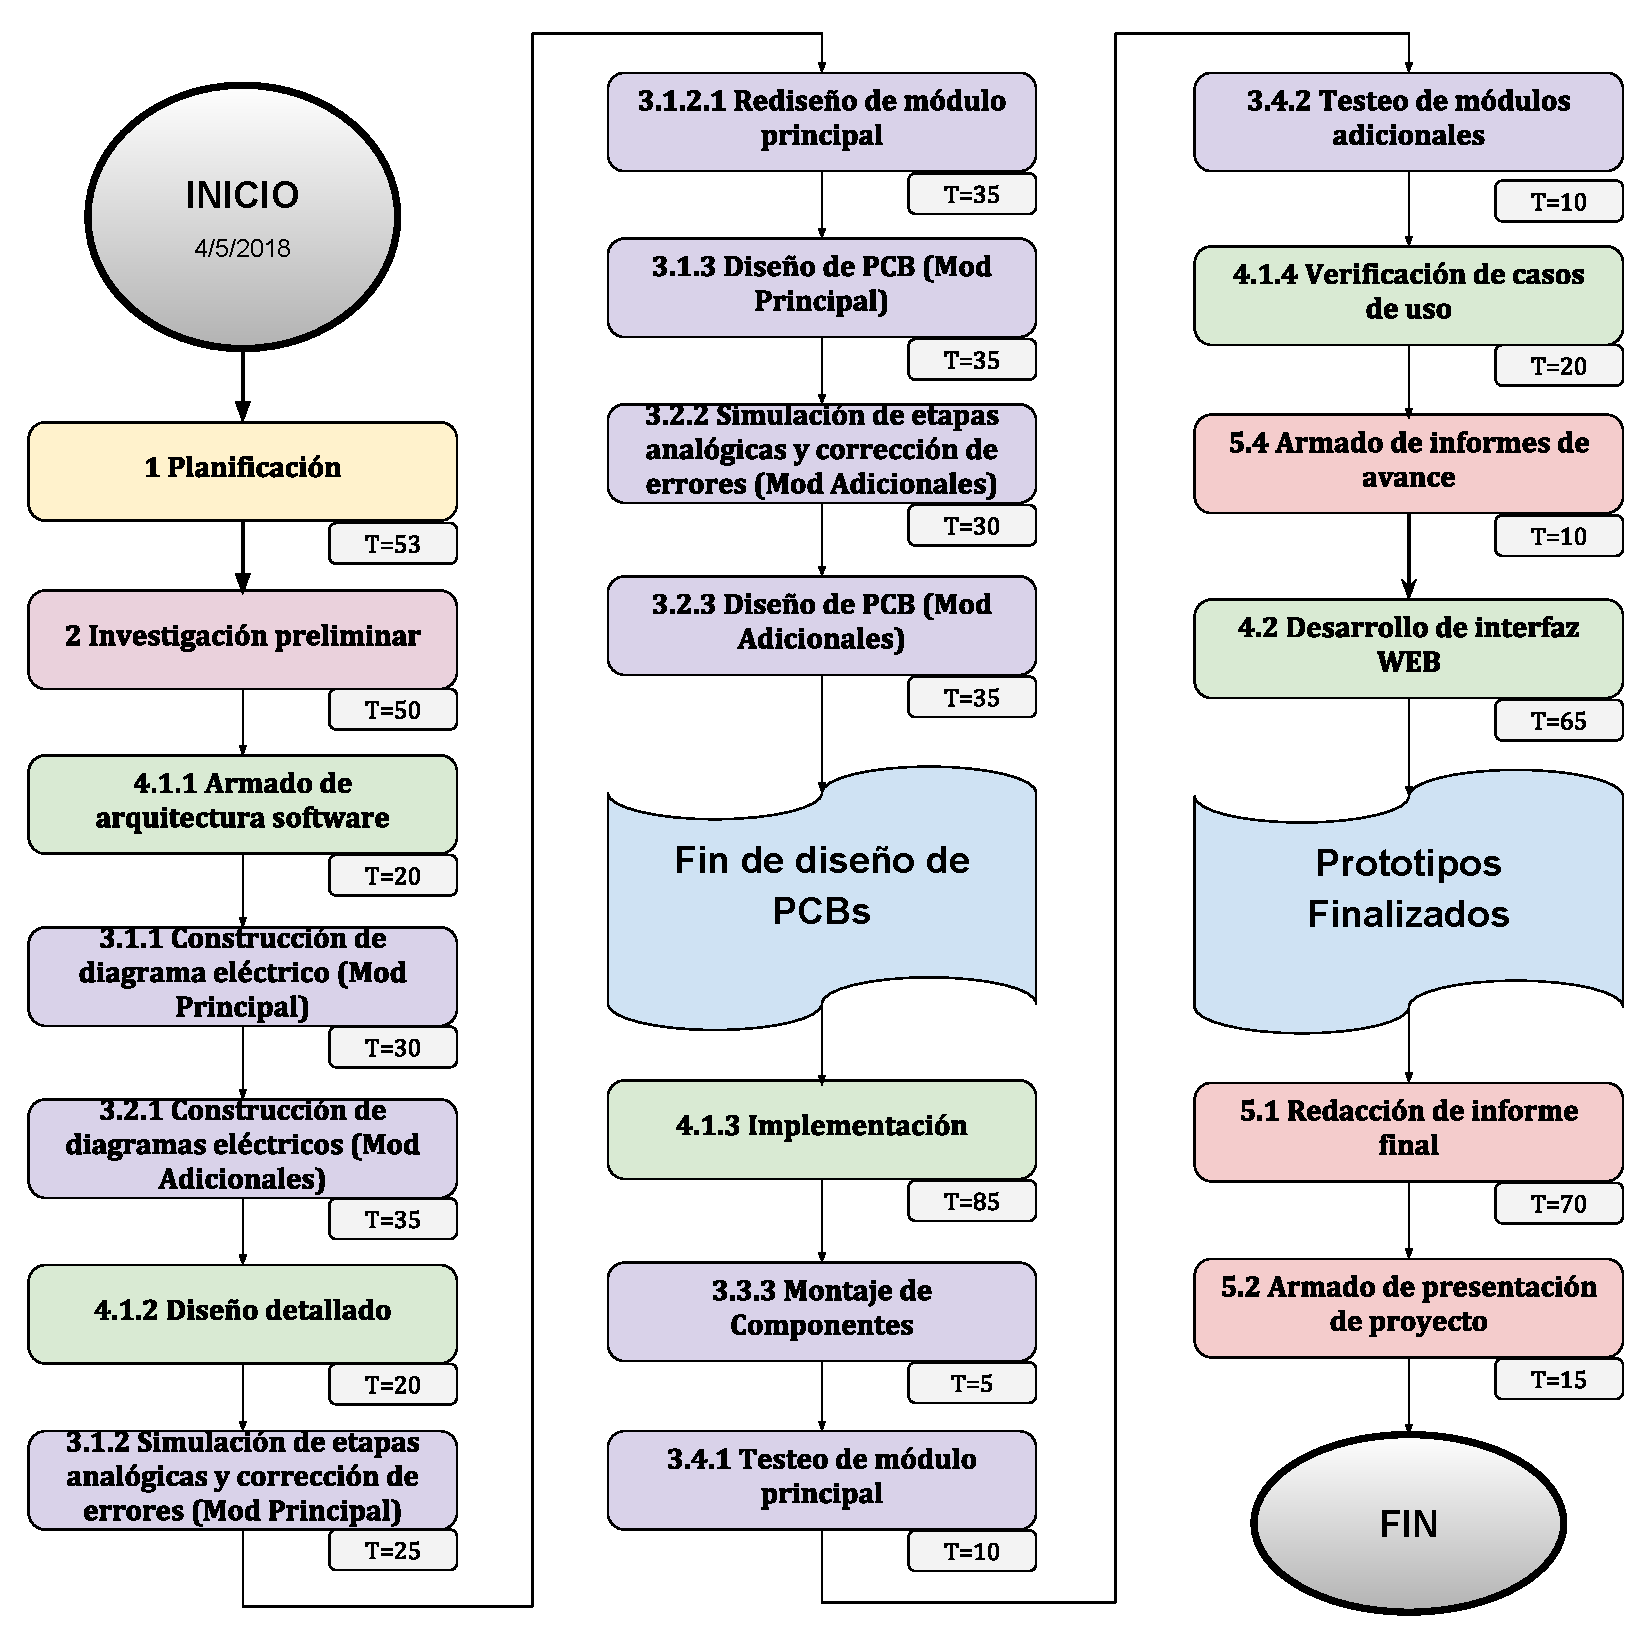
\includegraphics[width=1\textwidth]{./DiagramaAON.pdf}
	\caption{Diagrama activity on node del trabajo.}
	\label{fig:AON}
\end{figure}

\section{Módulo WIFI ESP-01}
Uno de los requerimientos establecidos para el trabajo final fue dotar al equipo probador de una conexión WIFI para la implementación de la interfaz de usuario. Para dicho fin se utilizó un módulo WIFI modelo ESP-01, desarrollado por la empresa AI-Thinker. En la figura \ref{fig:ESP01} se puede ver una fotografía del módulo.

\begin{figure}[H]
	\centering
	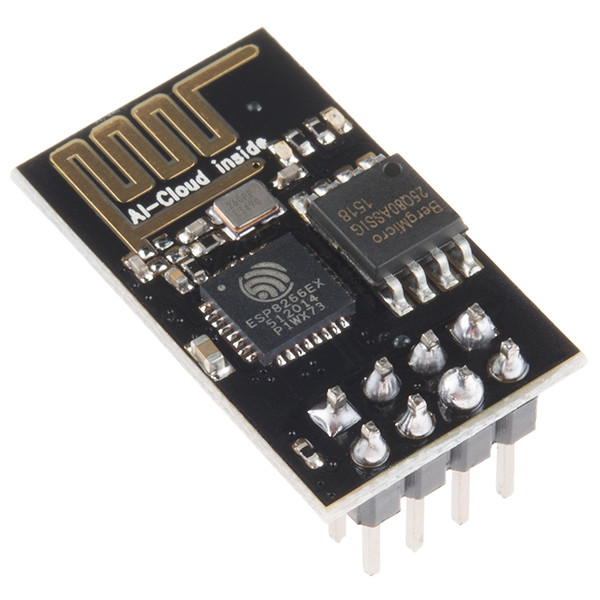
\includegraphics[width=0.4\textwidth]{./ESP-01.jpg}
	\caption{Módulo WIFI ESP-01 de AI Thinker\protect\footnotemark.}
	\label{fig:ESP01}
\end{figure}
\footnotetext{Imagen tomada de \url{https://es.wikipedia.org/wiki/ESP8266}}


El módulo ESP-01 es un dispositivo basado en el SoC (\emph{System on Chip}, sitema en chip) ESP8266EX fabricado por Espressif \citep{ESP01}, cuyas principales características son:
\begin{itemize}
	\item Núcleo Tensilica L106 de 32 bit funcionando a 80 Mhz.
	\item Stack TCP/IP y WIFI integrado.
	\item Compatible con estándar IEEE 802.11b/g/n .
	\item Seguridad WEP/WPA-PSK/WPA2-PSK.
	\item Posibilidad de funcionamiento en modo \emph{station}, \emph{access point} y \emph{station+access point}.
	\item Configuración y comunicación mediante comandos AT por interfaz UART.
	\item Cuatro GPIOs disponibles, de los cuales dos son para la interfaz UART.

\end{itemize}

Si bien el módulo ESP-01 resuelve una parte de la comunicación estableciendo las conexiones y enviando y recibiendo paquetes de datos, es necesario montar un servidor que sea capaz de resolver las distintas peticiones de datos o recursos que lleguen a través del módulo. Para esto se utiliza el protocolo HTTP que se verá a continuación. 

\section{Protocolo HTTP}

El protocolo de transferencia de hipertexto, conocido como HTTP, es un protocolo de comunicación que permite el intercambio o acceso a datos y recursos entre dispositivos servidores y clientes. Este protocolo es la base del intercambio de datos en la web\citep{HTTPWIKI}.
 
Un uso muy habitual del protocolo HTTP es la carga de una página Web, donde el navegador Web actúa de cliente iniciando la comunicación y solicita a un servidor un recurso, por ejemplo una página Web. Esta solicitud se realiza mediante una petición HTTP con una estructura básica, como se ve en la figura \ref{fig:HTTP_Req}, que incluye:
\begin{itemize}
	\item Un método que indica al servidor qué es lo que se pretende hacer con la petición HTTP\citep{HTTPMOZI}. Los métodos más usados son GET, para obtener un recurso del servidor, y POST para enviar información desde el cliente al servidor.
	\item La URL, que indica la ubicación del recurso al que se quiere acceder en el servidor.
	\item La versión del protocolo HTTP que se está utilizando.
	\item Una cabecera que opcionalmente se puede incluir con distintos parámetros, por ejemplo lenguaje aceptado, tipo de contenido, fecha y hora, datos del navegador, etc. 
	\item El cuerpo del mensaje, normalmente utilizado en métodos POST para enviar información al servidor.
\end{itemize}

\begin{figure}[H]
	\centering
	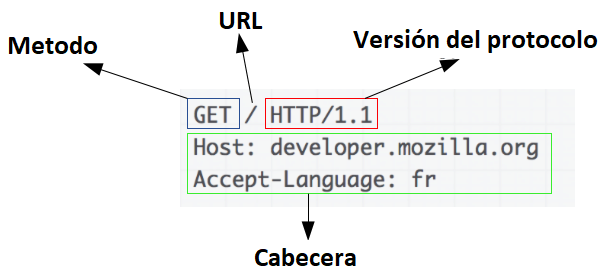
\includegraphics[width=1\textwidth]{./HTTP_Request.png}
	\caption{Estructura de una petición HTTP\protect\footnotemark.}
	\label{fig:HTTP_Req}
\end{figure}
\footnotetext{Imagen tomada de \url{https://developer.mozilla.org/es/docs/Web/HTTP/Overview}}


Luego, el servidor puede responder con los datos pedidos por el cliente, que al tratarse de la carga de una página Web, es habitual que ésta se realice por partes, transfiriendo documentos HTML, scripts, hojas de estilo y datos.

Al igual que las peticiones HTTP, las respuestas HTTP también tienen una estructura, como se ve en la figura \ref{fig:HTTP_Resp}, compuesta por:

\begin{itemize}
	\item La versión del protocolo.
	\item El código del estado, es decir un código que indica si se pudo ejecutar la solicitud y en caso contrario por qué no se pudo.
	\item Mensaje de estado.
	\item Una cabecera con parámetros al igual que en la petición.
	\item El cuerpo con el recurso pedido.
\end{itemize}

\begin{figure}[H]
	\centering
	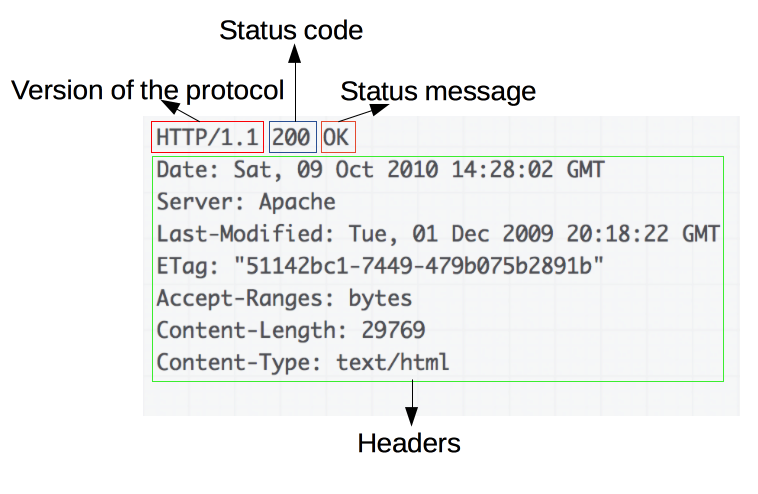
\includegraphics[width=1\textwidth]{./HTTP_Response.png}
	\caption{Estructura de una respuesta HTTP\protect\footnotemark.}
	\label{fig:HTTP_Resp}
\end{figure}
\footnotetext{Imagen tomada de \url{https://developer.mozilla.org/es/docs/Web/HTTP/Overview}}

Finalmente, el cliente, que en este caso es un navegador Web, compone la página web y ejecuta los scripts.

